% Options for packages loaded elsewhere
\PassOptionsToPackage{unicode}{hyperref}
\PassOptionsToPackage{hyphens}{url}
%
\documentclass[
]{article}
\usepackage{amsmath,amssymb}
\usepackage{iftex}
\ifPDFTeX
  \usepackage[T1]{fontenc}
  \usepackage[utf8]{inputenc}
  \usepackage{textcomp} % provide euro and other symbols
\else % if luatex or xetex
  \usepackage{unicode-math} % this also loads fontspec
  \defaultfontfeatures{Scale=MatchLowercase}
  \defaultfontfeatures[\rmfamily]{Ligatures=TeX,Scale=1}
\fi
\usepackage{lmodern}
\ifPDFTeX\else
  % xetex/luatex font selection
\fi
% Use upquote if available, for straight quotes in verbatim environments
\IfFileExists{upquote.sty}{\usepackage{upquote}}{}
\IfFileExists{microtype.sty}{% use microtype if available
  \usepackage[]{microtype}
  \UseMicrotypeSet[protrusion]{basicmath} % disable protrusion for tt fonts
}{}
\makeatletter
\@ifundefined{KOMAClassName}{% if non-KOMA class
  \IfFileExists{parskip.sty}{%
    \usepackage{parskip}
  }{% else
    \setlength{\parindent}{0pt}
    \setlength{\parskip}{6pt plus 2pt minus 1pt}}
}{% if KOMA class
  \KOMAoptions{parskip=half}}
\makeatother
\usepackage{xcolor}
\usepackage[margin=1in]{geometry}
\usepackage{graphicx}
\makeatletter
\def\maxwidth{\ifdim\Gin@nat@width>\linewidth\linewidth\else\Gin@nat@width\fi}
\def\maxheight{\ifdim\Gin@nat@height>\textheight\textheight\else\Gin@nat@height\fi}
\makeatother
% Scale images if necessary, so that they will not overflow the page
% margins by default, and it is still possible to overwrite the defaults
% using explicit options in \includegraphics[width, height, ...]{}
\setkeys{Gin}{width=\maxwidth,height=\maxheight,keepaspectratio}
% Set default figure placement to htbp
\makeatletter
\def\fps@figure{htbp}
\makeatother
\setlength{\emergencystretch}{3em} % prevent overfull lines
\providecommand{\tightlist}{%
  \setlength{\itemsep}{0pt}\setlength{\parskip}{0pt}}
\setcounter{secnumdepth}{-\maxdimen} % remove section numbering
\usepackage{float}
\floatplacement{figure}{H}
\ifLuaTeX
  \usepackage{selnolig}  % disable illegal ligatures
\fi
\IfFileExists{bookmark.sty}{\usepackage{bookmark}}{\usepackage{hyperref}}
\IfFileExists{xurl.sty}{\usepackage{xurl}}{} % add URL line breaks if available
\urlstyle{same}
\hypersetup{
  pdftitle={Exploring why the models do not fit Boussard 2020 data so well},
  pdfauthor={Andrés E. Quiñones},
  hidelinks,
  pdfcreator={LaTeX via pandoc}}

\title{Exploring why the models do not fit Boussard 2020 data so well}
\author{Andrés E. Quiñones}
\date{2024-01-23}

\begin{document}
\maketitle

\hypertarget{the-boussard-et-al-data-set}{%
\subsection{\texorpdfstring{The Boussard \emph{et al} data
set}{The Boussard et al data set}}\label{the-boussard-et-al-data-set}}

In here I present the statistical model used to estimate reinforcement
learning parameters from data from a reversal learning task. In the
experimental set up, individuals from two experimental treatments are
trained to pick one of two stimuli. Where one of those two options
provides reward in the form of food pellets. The experiments is composed
of 11 reversal blocks, each of these blocks is composed of 30 trial. In
other words, every 30 trials the stimulus that provides reward is
switched. Thus, individuals must reverse their estimate of reward in
order to make adaptive decisions and choose the rewarding stimulus. In
figure \ref{fig:plotBoussard}, I show the proportion of correct choices
for both treatment groups along the trials, and reversal blocks.

\begin{figure}

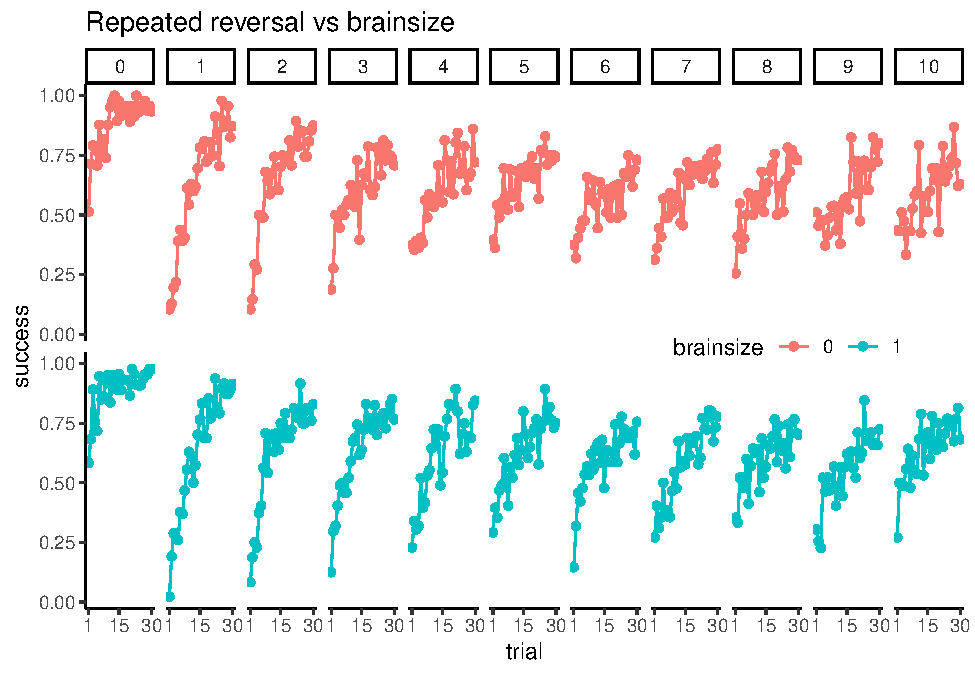
\includegraphics{report_boussard2020_files/figure-latex/plotBoussard-1} \hfill{}

\caption{The Boussard *et al* data-set. Points show the proportion of successes achieved by individuals of both treatment groups along trials and reversal blocks.}\label{fig:plotBoussard}
\end{figure}

\hypertarget{fitting-the-model-with-the-initial-block}{%
\subsection{Fitting the model with the initial
block}\label{fitting-the-model-with-the-initial-block}}

\begin{flushleft}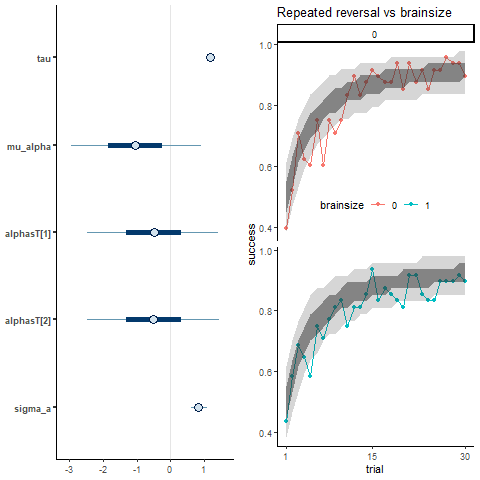
\includegraphics[width=6.67in,]{images/Boussard_short_0_alpha} \end{flushleft}

\hypertarget{the-initial-block-with-a-model-that-allows-flexible-learning-rates}{%
\subsection{The initial block with a model that allows flexible learning
rates}\label{the-initial-block-with-a-model-that-allows-flexible-learning-rates}}

\begin{flushleft}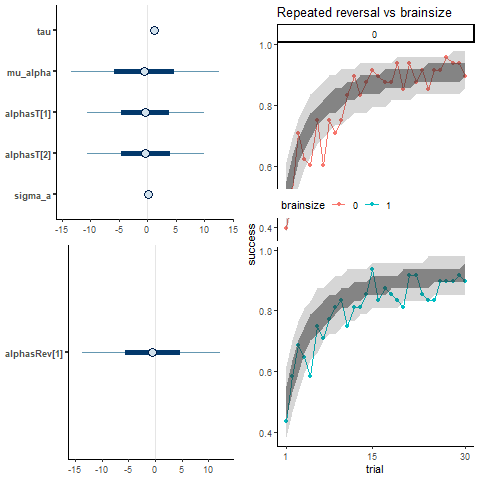
\includegraphics[width=6.67in,]{images/boussard_short_0_rev} \end{flushleft}

\hypertarget{the-initial-block-with-a-model-that-allows-flexible-learning-rates-for-two-blocks}{%
\subsection{The initial block with a model that allows flexible learning
rates for two
blocks}\label{the-initial-block-with-a-model-that-allows-flexible-learning-rates-for-two-blocks}}

\begin{flushleft}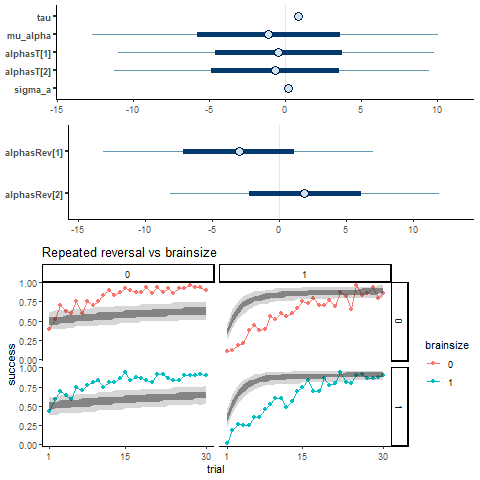
\includegraphics[width=6.67in,]{images/boussard_short_01_rev} \end{flushleft}

\hypertarget{fitting-a-model-with-the-temperature-parameter-as-a-fixed-effect}{%
\subsection{Fitting a model with the temperature parameter as a fixed
effect}\label{fitting-a-model-with-the-temperature-parameter-as-a-fixed-effect}}

\begin{flushleft}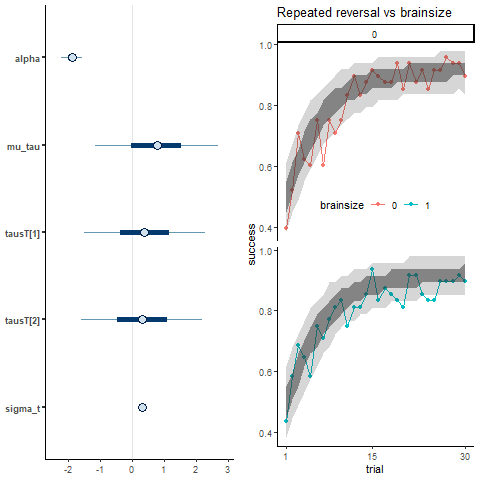
\includegraphics[width=6.67in,]{images/boussard_short_0_tau} \end{flushleft}

\hypertarget{fitting-a-model-with-different-tau-for-each-reversal-block-just-2-blocks}{%
\subsection{\texorpdfstring{Fitting a model with different \(\tau\) for
each reversal block (just 2
blocks)}{Fitting a model with different \textbackslash tau for each reversal block (just 2 blocks)}}\label{fitting-a-model-with-different-tau-for-each-reversal-block-just-2-blocks}}

\begin{flushleft}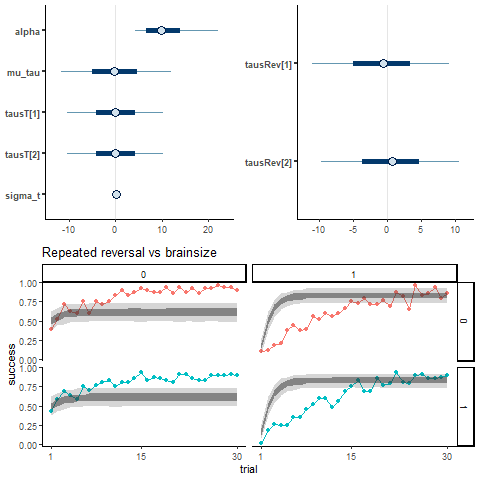
\includegraphics[width=6.67in,]{images/boussard_short_01_tau} \end{flushleft}

\hypertarget{fitting-a-model-with-a-different-tau-and-alpha-for-each-reversal-block}{%
\subsection{\texorpdfstring{Fitting a model with a different \(\tau\)
and \(\alpha\) for each reversal
block}{Fitting a model with a different \textbackslash tau and \textbackslash alpha for each reversal block}}\label{fitting-a-model-with-a-different-tau-and-alpha-for-each-reversal-block}}

\begin{flushleft}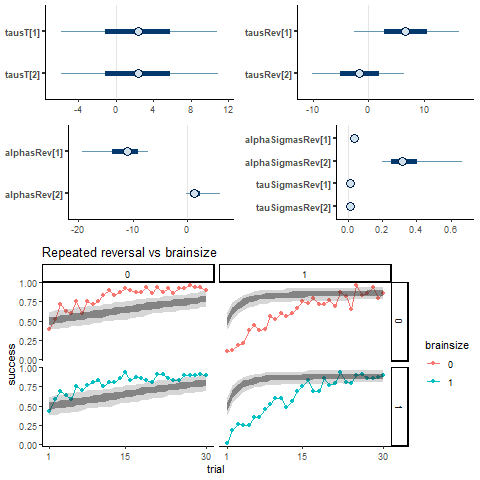
\includegraphics[width=6.67in,]{images/Boussard_short_alpha_tau_sigma} \end{flushleft}

\end{document}
